\documentclass[12pt, psamsfonts]{amsart}

%-------Packages---------
\usepackage{amssymb,amsfonts}
\usepackage{semantic}
\usepackage{fullpage}
\usepackage{tikz-cd}
\usepackage{todonotes}
\usepackage{physics}
\usepackage[all,arc]{xy}
\usepackage{enumerate}
\usepackage{enumitem}
\usepackage{mathrsfs}
\usepackage{theoremref}
\usepackage{graphicx}
\usepackage[bookmarks]{hyperref}

\usepackage{amsthm}
\makeatletter
\def\th@plain{%
  \thm@notefont{}% same as heading font
  \itshape % body font
}
\def\th@definition{%
  \thm@notefont{}% same as heading font
  \normalfont % body font
}
\makeatother

%--------Theorem Environments--------
%theoremstyle{plain} --- default
\newtheorem{thm}{Theorem}[subsection]
\newtheorem{cor}[thm]{Corollary}
\newtheorem{prop}[thm]{Proposition}
\newtheorem{lem}[thm]{Lemma}
\newtheorem{conj}[thm]{Conjecture}
\newtheorem{quest}[thm]{Question}

\theoremstyle{definition}
\newtheorem{defn}[thm]{Definition}
\newtheorem{defns}[thm]{Definitions}
\newtheorem{con}[thm]{Construction}
\newtheorem{exmp}[thm]{Example}
\newtheorem{exmps}[thm]{Examples}
\newtheorem{notn}[thm]{Notation}
\newtheorem{notns}[thm]{Notations}
\newtheorem{addm}[thm]{Addendum}
\newtheorem*{exer}{Exercise}

\theoremstyle{remark}
\newtheorem{rem}[thm]{Remark}
\newtheorem{rems}[thm]{Remarks}
\newtheorem{warn}[thm]{Warning}
\newtheorem{sch}[thm]{Scholium}

\DeclareMathOperator{\weight}{weight}
\DeclareMathOperator{\neighbors}{neighbors}
\DeclareMathOperator{\priority}{priority}


\makeatletter
\makeatother
\numberwithin{equation}{subsection}

\bibliographystyle{plain}

\setcounter{tocdepth}{3}
\makeatletter
\def\l@subsection{\@tocline{2}{0pt}{2.5pc}{5pc}{}}
\makeatother

\begin{document}

\title{Stellar Consensus Protocol}
\author{Hidenori Shinohara}

\maketitle

\tableofcontents
\pagebreak

\section{Federated Byzantine Agreement System}
\pagebreak

\subsection{Quorums}

\begin{defn}[Federated Byzantine Agreement System]
    Let $V$ be a set and $Q:V \rightarrow 2^{2^V} \setminus \{ \emptyset \}$ be a function such that $\forall v \in V, \forall q \in Q(v), v \in q$.
    Then we call the pair $\ev{V, Q}$ a federated Byzantine agreement system, or FBAS for short.
    Each $q$ in $Q(v)$ is called a quorum slice for each $v \in V$.
\end{defn}

\begin{rem}\label{rem_fbas}
    $ $
    \begin{itemize}
        \item
            For each node $v$, $Q(v)$ is a set of subsets of $V$.
            For instance, node $v_1$ may trust $v_2, v_3, v_4$ and may have $\{ v_1, v_2, v_3, v_4 \} \in Q(v_1) \subset 2^V$.
        \item
            Note that we explicitly exclude $\emptyset$ from the co-domain.
            In other words, we want $Q(v) \ne \emptyset$ for all $v \in V$.
            If $Q(v) = \emptyset$ for some $v \in V$, it satisfies $\forall q \in Q(v), v \in q$.
            As we will see, each $q \in Q(v)$ is the list of nodes that $v$ trusts.
            If $v$ has no list of nodes that it trusts, $v$ cannot really do anything.
            Thus we want $Q(v) \ne \emptyset$ for all $v \in V$.
        \item
            Consider the case when $V = \emptyset$.
            Note that $2^\emptyset = \{ \emptyset \}$ and thus $2^{2^\emptyset} = \{ \emptyset, \{ \emptyset \} \}$.
            Thus $V$ forms an FBAS where $Q$ is the map $\emptyset \mapsto \{ \{ \emptyset \} \}$.
    \end{itemize}
\end{rem}

\begin{defn}[Quorum]
    Let $\ev{V, Q}$ be an FBAS\@.
    $U \subset V$ is called a quorum if and only if $U \ne \emptyset$ and $\forall v \in U, \exists q \in Q(v), q \subset U$.
\end{defn}

\begin{thm}\label{union_quorums}
    In an FBAS $\ev{V, Q}$, the union of two quorums is a quorum.
\end{thm}

\begin{proof}
    Let $U_1, U_2$ be two quorums.
    Let $v \in U_1 \cup U_2$.
    Then $v \in U_i$ for $i = 1$ or $i = 2$.
    Then $q \subset U_i$ for some $q \in Q(v)$.
    Therefore, $q \subset U_1 \cup U_2$, so $U_1 \cup U_2$ is indeed a quorum.
\end{proof}

\begin{cor}
    The set of quorums of a given FBAS is closed under union.
\end{cor}

\begin{thm}
    In an FBAS $\ev{V, Q}$, $V$ is a quorum.
\end{thm}

\begin{proof}
    For any $v \in V$, for any $q \in Q(v)$, $q \subset V$.
    Therefore, $V$ is indeed a quorum.
\end{proof}

\begin{exmp}
    One might wonder if the intersection of quorums is always a quorum.
    However, this is not true in general.

    Let $V = \{ v_1, \ldots, v_4 \}$ and
    \begin{itemize}
        \item
            $Q(v_1) = \{ \{ v_1, v_2, v_3 \}, \{ v_1, v_2, v_4 \}, \{ v_1, v_3, v_4 \} \}$,
        \item
            $\vdots$
        \item
            $Q(v_4) = \{ \{ v_1, v_2, v_4 \}, \{ v_1, v_3, v_4 \}, \{ v_2, v_3, v_4 \} \}$.
    \end{itemize}

    In other words, $Q(v_i) = \{ U \subset V \mid \abs{U} = 3, v_i \in U \}$.

    Then $U_1 = \{ v_1, v_2, v_3 \}$ is a quorum, and $U_2 = \{ v_2, v_3, v_4 \}$ is a quorum.
    However, $U_1 \cap U_2 = \{ v_2, v_3 \}$ is not a quorum because the size of any quorum slice is 3.
\end{exmp}

\begin{defn}[Quorum Intersection]
    Let $\ev{V, Q}$ be an FBAS\@.
    We say $\ev{V, Q}$ enjoys quorum intersection if and only if $U_1 \cap U_2 \ne \emptyset$ for any pair of quorums $U_1, U_2$.
\end{defn}

\begin{defn}[Delete]\label{delete_fbas}
    Let $\ev{V, Q}$ be an FBAS and $B \subset V$.
    Then the FBAS $\ev{V, Q}^B$ is defined to be $\ev{V \setminus B, Q^B}$ where $\forall v \in V \setminus B, Q^B(v) = \{ q \setminus B \mid q \in Q(v) \}$.
\end{defn}

\begin{rem}
    One may think that this is related to fail-stop behaviors where $B$ is the set of nodes that stopped responding.
    In general, however, this is not true as we also remove nodes from quorum slices.
    One can think of this as the \textit{alternate} universe where nodes from $B$ simply did not even exist from the beginning.
\end{rem}

\begin{thm}
    Definition~\ref{delete_fbas} is well-defined.
    In other words, if $\ev{V, Q}$ is an FBAS and $B \subset V$, then $\ev{V, Q}^B$ is an FBAS\@.
\end{thm}

\begin{proof}
    If $V = B$, then we are done because of Remark~\ref{rem_fbas}.

    Suppose otherwise.
    Let $v \in V \setminus B$ be given.
    By the definition of an FBAS, $Q(v) \ne \emptyset$.
    Therefore, $Q^B(v) = \{ q \setminus B \mid q \in Q(v) \}$ is nonempty.

    Let $q' \in Q^B(v)$ be given arbitrarily.
    Then $q' = q \setminus B$ for some $q \in Q(v)$.
    Then $v \in q$ by the definition of an FBAS, so $v \in q'$.
    
    Thus $Q^B$ is indeed a quorum function.
    Therefore, $\ev{V, Q}^B$ is an FBAS\@.
\end{proof}

\begin{thm}\label{quorum_delete_fbas}
    Let $U$ be a quorum in FBAS $\ev{V, Q}$, let $B \subset V$ be a set of nodes, and let $U' = U \setminus B$.
    If $U' \ne \emptyset$, then $U'$ is a quorum in $\ev{V, Q}^B$.
\end{thm}

\begin{proof}
    Since $U' \ne \emptyset$, it suffices to show that $\forall v \in U', \exists q \in Q^B(v), q \subset U'$.
    Let $v \in U'$.
    Then $v \in U$.
    Since $U$ is a quorum in $\ev{V, Q}$, we can find $q \in Q(v)$ such that $q \subset U$.
    Then $q' = q \setminus B \in Q^B(v)$, and $q' = q \setminus B \subset U \setminus B = U'$.
    Therefore, $U'$ is a quorum in $\ev{V, Q}^B$.
\end{proof}

\begin{rem}
    One can think of this theorem as ``\textit{A quorum in the `original' universe is a quorum in the `alternate' universe.}"
\end{rem}

\begin{defn}[Quorum Intersection Despite $B$]
    Let $\ev{V, Q}$ be an FBAS and $B \subset V$ be a set of nodes.
    We say $\ev{V, Q}$ enjoys quorum intersection despite $B$ if and only if $\ev{V, Q}^B$ enjoys quorum intersection.
\end{defn}

\begin{rem}
    Quorum intersection despite $B$ is related to the system-level safety when nodes in $B$ act arbitrarily.
    For instance, suppose $\ev{V, Q}$ is an FBAS, $B$ is the set of all ill-behaved nodes, and $\ev{V, Q}$ enjoys quorum intersection despite $B$.
    Suppose two well-behaved nodes $v_1, v_2$ agree with contradictory statements $a_1, a_2$ in quorums $q_1, q_2$, respectively.
    \todo[inline,caption={}]{
        Rewrite this!
    }
    Then $q_1 \cap q_2 \ne \emptyset$ have well-behaved nodes who agreed with both $a_1$ and $a_2$.
    This is a contradiction because a well-behaved node cannot contradict itself.
    This example illustrates how the concept of quorum intersection despite $B$ is related to system-level safety when nodes in $B$ experience Byzantine failures.
\end{rem}

\begin{defn}[Quorum Availability Despite $B$]\label{def_quorum_availability}
    Let $\ev{V, Q}$ be an FBAS and $B \subset V$ be a set of nodes.
    We say $\ev{V, Q}$ enjoys quorum availability despite $B$ if and only if $V \setminus B$ is a quorum in $\ev{V, Q}$ or $B = V$.
\end{defn}

\begin{thm}\label{quorum_availability_equivalence_condition}
    Let $\ev{V, Q}$ be an FBAS and $B \subset V$.
    $\ev{V, Q}$ enjoys quorum availability despite $B$ if and only if $\forall v \in V \setminus B$, there exists a quorum $U_v$ such that $v \in U_v \subset (V \setminus B)$.
\end{thm}

\begin{proof}
    If $V = B$, we are done.
    Suppose otherwise.
    \begin{align*}
        \forall v \in V \setminus B, \exists \text{a quorum $U_v$}, v \in U_v \subset (V \setminus B)
            &\implies \bigcup_{v \in V \setminus B} U_v \text{ is a quorum in $\ev{V, Q}$} \\
            &\implies \text{$V \setminus B$ is a quorum in $\ev{V, Q}$}
    \end{align*}
    by Theorem~\ref{union_quorums}.
    On the other hand, if $V \setminus B$ is a quorum in $\ev{V, Q}$, then $\forall v \in V \setminus B, \exists \text{a quorum $U_v$}, v \in U_v \subset (V \setminus B)$ because we can let $U_v = V \setminus B$ for each $v$.
\end{proof}

\begin{rem}
    Theorem~\ref{quorum_availability_equivalence_condition} shows that $\ev{V, Q}$ enjoys quorum availability despite $B$ if all nodes in $V \setminus B$ can find a quorum without $B$.
    This is related to the liveness of the system.
    If $\ev{V, Q}$ enjoys quorum availability despite $B$, then regardless of what happens to nodes in $B$, nodes in $V \setminus B$ can keep going.
\end{rem}

\begin{defn}[$v$-blocking]\label{def_v_blocking}
    Let $\ev{V, Q}$ be an FBAS\@.
    Let $v \in V$.
    A subset $B \subset V$ is called $v$-blocking if and only if $\forall q \in Q(v), q \cap B \ne \emptyset$.
\end{defn}

\begin{rem}
    Intuitively, if a subset $B \subset V$ is $v$-blocking, then one may think of it as ``\textit{$v$ can't really get by without $B$}."
    The following theorem can be interpreted as ``\textit{If $v$ can't get by without $B$, $v$ can't get by without $C$ for any $C \supset B$}."
\end{rem}

\begin{thm}\label{basic_prop_v_blocking}
    Let $\ev{V, Q}$ be an FBAS\@.
    Let $v \in V$.
    Then
    \begin{itemize}
        \item
            The union of two $v$-blocking sets is $v$-blocking.
        \item
            Any superset of a $v$-blocking set is $v$-blocking.
    \end{itemize}
\end{thm}

\begin{proof}
    It suffices to only prove the second statement.
    If $B \subset B'$ and $B$ is $v$-blocking, $q \cap B' \supset q \cap B \ne \emptyset$ for any $q \in Q(v)$.
\end{proof}

\begin{thm}\label{v_blocking_delete}
    Let $\ev{V, Q}$ be an FBAS\@.
    Let $A \subsetneq V$ and $U_1, U_2$ be a partition of $V \setminus A$.
    Let $v \in U_1$.
    If $U_2$ is not $v$-blocking in $\ev{V, Q}$, then $U_2$ is not $v$-blocking in $\ev{V, Q}^A$.
\end{thm}

\begin{proof}
    Since $U_2$ is not $v$-blocking in $\ev{V, Q}$, there exists $q_v \in Q(v)$ such that $q_v \cap U_2 = \emptyset$.
    \begin{align*}
        (q_v \setminus A) \cap U_2
            &= (q_v \cap U_2) \setminus (A \cap U_2) \\
            &= q_v \cap U_2 = \emptyset.
    \end{align*}
    Thus $U_2$ is not $v$-blocking in $\ev{V, Q}^A$.
\end{proof}

\begin{thm}\label{quorum_availability_v_blocking}
    Let $\ev{V, Q}$ be an FBAS\@.
    Let $B \subset V$.
    $\ev{V, Q}$ enjoys quorum availability despite $B$ if and only if $B$ is not $v$-blocking for any $v \in V \setminus B$.
\end{thm}

\begin{proof}
    \begin{align*}
        \forall v \in V \setminus B, \neg(\text{$B$ is $v$-blocking})
            &\iff \forall v \in V \setminus B, \neg(\forall q \in Q(v), q \cap B \ne \emptyset) \\
            &\iff \forall v \in V \setminus B, \exists q \in Q(v), q \cap B = \emptyset \\
            &\iff \forall v \in V \setminus B, \exists q \in Q(v), q \subset V \setminus B \\
            &\iff \text{$V = B$ or $V \setminus B$ is a quorum in $\ev{V, Q}$} \\
            &\iff \text{$\ev{V, Q}$ enjoys quorum availability despite $B$}
    \end{align*}
\end{proof}

\newpage
\subsection{Dispensable Sets}

\begin{defn}[Dispensable Set]\label{def_dset}
    Let $\ev{V, Q}$ be an FBAS and $B \subset V$ be a set of nodes.
    $B$ is called a dispensable set, or DSet, if and only if $\ev{V, Q}$ enjoys both quorum intersection despite $B$ and quorum availability despite $B$.
\end{defn}

We will first show some basic properties of DSets.
\begin{thm}
    Let $\ev{V, Q}$ be an FBAS.
    Then
    \begin{itemize}
        \item
            $V$ is a DSet.
        \item
            If $\forall v \in V, Q(v) = \{ V \}$, then $\emptyset$ and $V$ are the only DSets of $\ev{V, Q}$.
    \end{itemize}
\end{thm}

\begin{proof}
    $ $
    \begin{itemize}
        \item
            $\ev{V, Q}^V$ enjoys quorum intersection because there is no quorum.
            $\ev{V, Q}$ enjoys quorum availability despite $V$ because $V = V$.
        \item
            Suppose $\forall v \in V, Q(v) = \{ V \}$.
            As shown above, $V$ is a DSet of $\ev{V, Q}$.
            The empty set is a DSet because
            \begin{itemize}
                \item
                    $\ev{V, Q}$ enjoys quorum intersection despite $\emptyset$ because the only quorum is $V$.
                \item
                    $\ev{V, Q}$ enjoys quorum availability despite $B$ because $V \setminus \emptyset = V$ is a quorum.
            \end{itemize}
            Let $\emptyset \subsetneq S \subsetneq V$ be given.
            Then $V \ne S$ and $V \setminus S$ is not a quorum for it is nonempty and does not contain any quorum slice.
            Therefore, $\ev{V, Q}$ does not enjoy quorum availability despite $B$, so no nonempty, proper subset of $V$ is a DSet.
    \end{itemize}
\end{proof}

\begin{defn}[Intact and Befouled]\label{def_intact_befouled}
    Let $\ev{V, Q}$ be an FBAS and $v \in V$.
    $v$ is said to be intact if and only if there exists a DSet $B$ containing all ill-behaved nodes and $v \notin B$.
    $v$ is said to be befouled if and only if $v$ is not intact.
\end{defn}

\begin{figure}[!htb]
    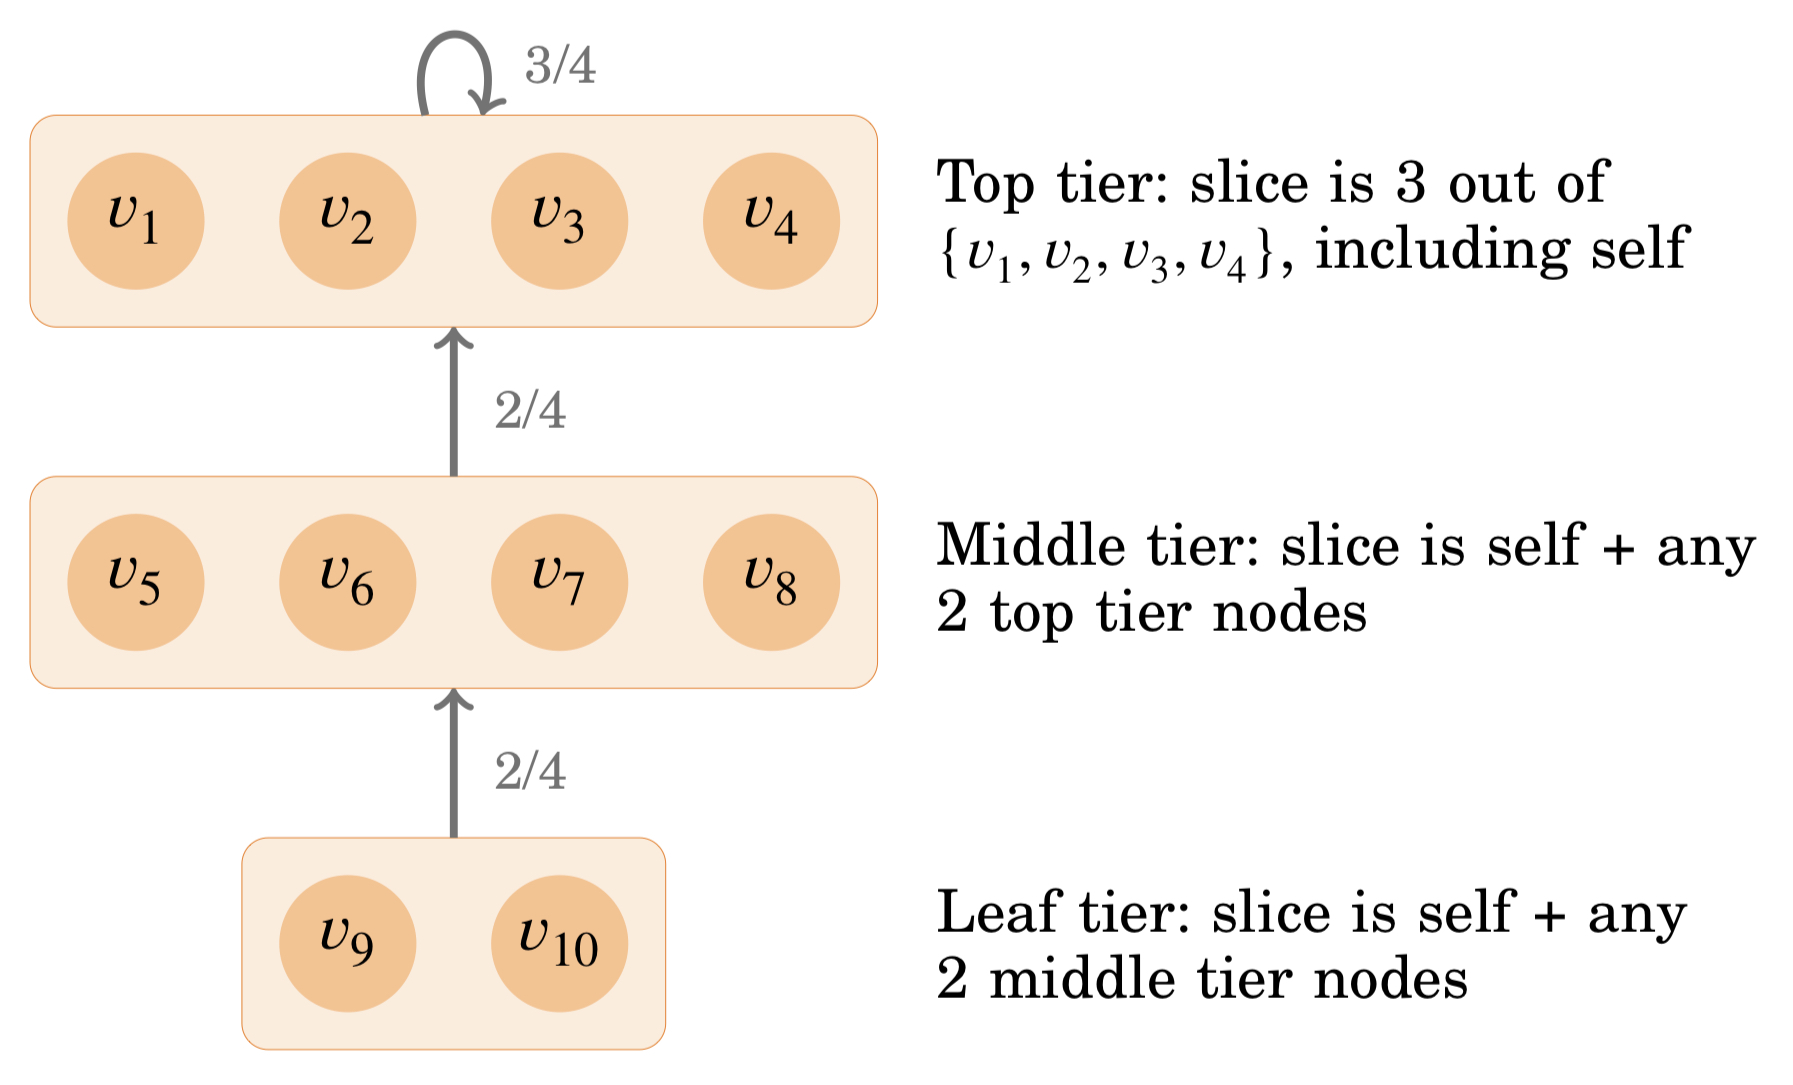
\includegraphics[width=.5\linewidth]{img/tiered_quorum_example.jpeg}
        \caption{Tiered Quroum Example (P.5 of the white paper)}
    \label{fig:tiered_quorum_example}
\end{figure}

\begin{exmp}
    We will use Figure~\ref{fig:tiered_quorum_example} as an example.

    \begin{itemize}
        \item
            The smallest DSet containing $v_5, v_6$ in Figure~\ref{fig:tiered_quorum_example} is $\{ v_5, v_6, v_9, v_{10} \}$.
            \begin{itemize}
                \item
                    First, we will show that $B = \{ v_5, v_6 \}$ is not a DSet.
                    By definition,
                    \begin{align*}
                        Q^B(v_9) &= \{ \{ v_9 \}, \{ v_9, v_7 \}, \{ v_9, v_8 \}, \{ v_9, v_7, v_8 \} \} \\
                        Q^B(v_{10}) &= \{ \{ v_{10} \}, \{ v_{10}, v_7 \}, \{ v_{10}, v_8 \}, \{ v_{10}, v_7, v_8 \} \}
                    \end{align*}
                    This implies that $U_9 = \{ v_9 \}$ and $U_{10} = \{ v_{10} \}$ are both quorums.
                    Then $U_9 \cap U_{10} = \emptyset$, so $\ev{V, Q}^B$ does not enjoy quorum intersection.
                    Therefore, $B$ is not a DSet.

                    Next, we will consider $C = \{ v_5, v_6, v_1 \}$.
                    Then we can use the same argument as above.
                    $U_9 = \{ v_9 \} \in Q^C(v_9)$ and $U_{10} = \{ v_{10} \} \in Q^C(v_{10})$, and the intersection is empty.
                    Therefore, $C$ is not a DSet.
                    It is easy to see that this argument works for the case of $\{ v_5, v_6, v_i \}$ for any $i = 1, 2, 3, 4$.

                    We will consider $D = \{ v_5, v_6, v_9 \}$.
                    Similarly, $U = \{ v_{10} \} \in Q^D(v_{10})$ is a quorum.
                    Moreover, $U' = \{ v_1, v_2, v_3, v_4 \}$ is a quorum.
                    Then $U \cap U' = \emptyset$, so $\ev{V, Q}^D$ does not enjoy quorum intersection.
                    It is easy to see that a similar argument shows that $\{ v_5, v_6, v_{10} \}$ is not a DSet.

                    Finally, we will show that $E = \{ v_5, v_6, v_9, v_{10} \}$ is a DSet.
                    $V \setminus E$ is a quorum in $\ev{V, Q}$ because every node in $V \setminus E$ has a quorum slice consisting of nodes in $V \setminus E$.
                    If a quorum in $\ev{V, Q}^E$ contains $v_7$ or $v_8$, then it must contain some of $v_1, v_2, v_3, v_4$.
                    If a quorum in $\ev{V, Q}^E$ contains at least one of $v_1, v_2, v_3$, or $v_4$, then it must contain at least three of $v_1, v_2, v_3, v_4$.
                    Therefore, any intersection of two quorums in $\ev{V, Q}^E$ contains at least two of $v_1, v_2, v_3, v_4$ by the pigeon hole principle.

                    Therefore, $E$ is indeed a smallest DSet containing $v_5$ and $v_6$.
                \item
                    We showed that $B = \{ v_5, v_6 \}$ is not a DSet because $\ev{V, Q}$ does not enjoy quorum intersection despite $B$.
                    What this means is that if both $v_5$ and $v_6$ either stop responding or are malicious, then it is not possible to guarantee safety for $v_9$ and $v_{10}$.
                    For instance, consider the following situation:
                    \begin{itemize}
                        \item
                            Both $v_5$ and $v_6$ tell $v_9$ and $v_{10}$ that $Q(v_5) = Q(v_6) = \{ \{ v_5, v_6 \} \}$ convincing that $\{ v_5, v_6, v_9 \}$ and $\{ v_5, v_6, v_{10} \}$ are both quorums.
                        \item
                            Both $v_5$ and $v_6$ tell $v_9$ that they want to process a certain transaction.
                            This transaction does not contradict what $v_9$ knows about $v_5$.
                            Moreover, everyone in the quorum $\{ v_5, v_6, v_9 \}$ is in favor of this transaction.
                            Thus there is no reason for $v_9$ to not believe this transaction.
                        \item
                            Both $v_5$ and $v_6$ tell $v_{10}$ that they want to process a certain transaction that contradicts the transaction they told $v_5$ about.
                            For the same reason, there is no reason for $v_{10}$ to not believe this transaction.
                        \item
                            Then the network processes contradicting transactions.
                            This can let $v_5$ double-spend some money, for instance.
                        \item
                            One can verify that this is possible by looking into the definition of accepting, confirming and such that are introduced in later chapters.
                    \end{itemize}
            \end{itemize}
        \item
            $B = \{ v_1 \}$ is a DSet.
            \begin{itemize}
                \item
                    First, we will check if $\ev{V, Q}$ enjoys quorum intersection despite $B$.

                    Consider $\ev{V, Q}^B$.
                    Any quorum containing $v_9$ and/or $v_{10}$ must contain at least two of $v_5, v_6, v_7, v_8$.
                    Any quorum containing at least one of $v_5, \cdots, v_8$ must contain at least one of $v_2, v_3, v_4$.
                    Any quorum containing at least one of $v_2, v_3, v_4$ must contain at least two of $v_2, v_3, v_4$.
                    This is because $Q(v_i)^B = \{ \{ v_2, v_3, v_4 \}, \{ v_i, v_j \}, \{ v_i, v_k \} \}$ where $\{ i, j, k \} = \{ 2, 3, 4 \}$.

                    Therefore, the intersection of any two quorums must contain at least one of $v_2, v_3, v_4$ by the pigeon hole principle.

                    Next, we need to check if $\ev{V, Q}$ enjoys quorum availability despite $B$.
                    $V \setminus B$ is indeed a quorum in $\ev{V, Q}$ because each node in $V \setminus B$ has a quorum slice that does not contain $v_1$.
                \item
                    We showed that $B$ is indeed a DSet.
                    What this means is that even if $v_1$ stops responding or becomes malicious, the rest of the network can make progress safely.
                    For instance, suppose that $v_1$ becomes malicious and tries to double-spend money.
                    $v_1$ might tell $v_5$ that it wants to process a certain transaction.
                    Similarly, $v_1$ might tell $v_6$ that it wants to process a contradicting transaction.
                    However, every quorum slice of $v_5$ and $v_6$ contains at least one tier-1 node that is not $v_1$.
                    Suppose that $v_5$ asks $v_2$ what it thinks, and $v_6$ asks $v_3$ what it thinks.
                    Then every quorum slice of $v_2$ and $v_3$ contains 3 tier-1 nodes.
                    By the pigeon hole principle, at least one tier-1 node that is not $v_1$ gets asked what it thinks about the contradicting transactions from $v_5$.
                    The tier-1 node does not agree with them and $v_1$'s attempt to double-spend money fails.
            \end{itemize}
    \end{itemize}
\end{exmp}

\begin{thm}\label{intersection_dset}
    If $B_1$ and $B_2$ are DSets in an FBAS $\ev{V, Q}$ enjoying quorum intersection, then $B = B_1 \cap B_2$ is a DSet, too.
\end{thm}

\begin{proof}
	If $B_1 = V$ or $B_2 = V$, then we are done.
	Suppose otherwise.

    First, we will show that $\ev{V, Q}$ enjoys quorum availability despite $B$.
    By Definition~\ref{def_quorum_availability}, it suffices to show that $V = B$ or $V \setminus B$ is a quorum in $\ev{V, Q}$.
    Since we assumed that $B_1 \ne V$ and $B_2 \ne V$, $B \ne V$.
    Therefore, we will show that $V \setminus B$ is a quorum in $\ev{V, Q}$.
    By basic set theory, $V \setminus B = V \setminus (B_1 \cap B_2) = (V \setminus B_1) \cup (V \setminus B_2)$.
    Since $B_1$ is a DSet, $V = B_1$ or $V \setminus B_1$ is a quorum in $\ev{V, Q}$.
    Since we assumed that $V \ne B_1$ earlier, $V \setminus B_1$ is a quorum in $\ev{V, Q}$.
    Similarly, $V \setminus B_2$ is a quorum in $\ev{V, Q}$.
    By Theorem~\ref{union_quorums}, the union $(V \setminus B_1) \cup (V \setminus B_2) = V \setminus B$ is a quorum in $\ev{V, Q}$.

    Next, we will show that $\ev{V, Q}$ enjoys quorum intersection despite $B$.
	Let $U_a, U_b$ be quorums in $\ev{V, Q}^B$.
    We want to show that $U_a \cap U_b \ne \emptyset$.
    We will do so by proving a stronger statement, which is $(U_a \cap U_b) \setminus B_1 \ne \emptyset$.
    In other words, we will show that $(U_a \setminus B_1) \cap (U_b \setminus B_1) \ne \emptyset$.

    Since $B_1$ is a DSet, $\ev{V, Q}$ enjoys quorum intersection despite $B_1$.
    In other words, $\ev{V, Q}^{B_1}$ enjoys quorum intersection.
    Therefore, it suffices to show that $U_a \setminus B_1$ and $U_b \setminus B_1$ are both quorums in $\ev{V, Q}^{B_1}$.
    By Theorem~\ref{quorum_delete_fbas}, $U_a \setminus B_1$ and $U_b \setminus B_1$ are quorums in $(\ev{V, Q}^B)^{B_1}$ if $U_a \setminus B_1 \ne \emptyset$ and $U_b \setminus B_1 \ne \emptyset$.
    Since $(\ev{V, Q}^B)^{B_1} = \ev{V, Q}^{B_1}$, it suffices to show that $U_a \setminus B_1 \ne \emptyset$ and $U_b \setminus B_1 \ne \emptyset$.
    
    We will first show that $U_a \setminus B_1 \ne \emptyset$.
    By basic set theory,
	\begin{align*}
        U_a &= U_a \setminus B \\
            &= U_a \setminus (B_1 \cap B_2) \\
            &= (U_a \setminus B_1) \cup (U_a \setminus B_2)
	\end{align*}
	because $U_a \cap B = \emptyset$.

	This implies that $(U_a \setminus B_1) \cup (U_a \setminus B_2) \ne \emptyset$.
    If $U_a \setminus B_1$ is nonempty, we are done.
    Suppose $U_a \setminus B_2$ is nonempty.
    We will show that this implies that $U_a \setminus B_1 \ne \emptyset$.
    We will do so by first finding two quorums in $\ev{V, Q}^{B_2}$ whose intersection is a subset of $U_a \setminus B_1$.
	Since $\ev{V, Q}^{B_2}$ enjoys quorum intersection, the intersection of such two quorums must be nonempty, which in turn shows that $U_a \setminus B_1$ is nonempty.

	\begin{itemize}
		\item
            We claim that $U_a \setminus B_2$ is a quorum in $\ev{V, Q}^{B_2}$.
            $U_a$ is a quorum in $\ev{V, Q}^B$.
            Since $U_a \setminus B_2$ is assumed to be nonempty, $U_a \setminus B_2$ is a quorum in $(\ev{V, Q}^B)^{B_2}$ by Theorem~\ref{quorum_delete_fbas}.
            Since $(\ev{V, Q}^B)^{B_2} = \ev{V, Q}^{B_2}$, $U_a \setminus B_2$ is a quorum in $\ev{V, Q}^{B_2}$.
		\item
            $V \setminus B_2 \ne \emptyset$ is a quorum in $\ev{V, Q}$ because $\ev{V, Q}$ must enjoy quorum availability despite $B_2$ and $B_2 \ne V$.
			Similarly, $V \setminus B_1 \ne \emptyset$ is a quorum in $\ev{V, Q}$.
			Because $\ev{V, Q}$ enjoys quorum intersection, $(V \setminus B_1) \cap (V \setminus B_2) \ne \emptyset$.
			In other words, $(V \setminus B_1) \setminus B_2 \ne \emptyset$.
            By applying Theorem~\ref{quorum_delete_fbas} to the fact that $V \setminus B_1$ is a quorum in $\ev{V, Q}$ and $(V \setminus B_1) \setminus B_2 \ne \emptyset$, we can conclude that $(V \setminus B_1) \setminus B_2$ is a quorum in $\ev{V, Q}^{B_2}$.
	\end{itemize}
	Since $\ev{V, Q}^{B_2}$ enjoys quorum intersection, $(U_a \setminus B_2) \cap ((V \setminus B_1) \setminus B_2) \ne \emptyset$.
	\begin{align*}
        \emptyset
            &\ne (U_a \setminus B_2) \cap ((V \setminus B_1) \setminus B_2) \\
            &= (U_a \cap (V \setminus B_1)) \setminus B_2 \\
            &\subset U_a \cap (V \setminus B_1) \\
            &= U_a \setminus B_1.
	\end{align*}
	Thus, $U_a \setminus B_1 \ne \emptyset$.

	The same argument will show that $U_b \setminus B_1 \ne \emptyset$.
\end{proof}

\begin{rem}
    Theorem~\ref{intersection_dset} states that the intersection of two DSets is a DSet if the FBAS enjoys quorum intersection.
    One might wonder if the union of two DSets is a DSet when the FBAS enjoys quorum intersection.
    However, this is not true in general.
    Consider the FBAS $\ev{V, Q}$ where $V = \{ v_1, v_2, v_3, v_4 \}$ and $Q(v_i) = \{ U \subset V \mid v_i \in U, \abs{U} = 3 \}$.
    This FBAS enjoys quorum intersection by the pigeon-hole principle because each quorum contains at least 3 elements.
    Then $B = \{ v_1 \}$ is a DSet because
    \begin{itemize}
        \item
            Quorum intersection despite $B$
            \begin{itemize}
                \item
                    Every quorum slice in $\ev{V, Q}^B$ contains at least 2 nodes because every quorum slice in $\ev{V, Q}$ contains exactly 3 nodes.
                    This implies that any quorum in $\ev{V, Q}^B$ must contain at least 2 nodes.
                    By the pigeon-hole principle, every pair of quorums in $\ev{V, Q}^B$ must intersect.
            \end{itemize}
        \item
            Quorum availability despite $B$
            \begin{itemize}
                \item
                    $V \setminus B = \{ v_2, v_3, v_4 \}$ is a quorum in $\ev{V, Q}$ because $\{ v_2, v_3, v_4 \} \in Q(v_i)$ for each $i = 2, 3, 4$.
            \end{itemize}
    \end{itemize}
    Similarly, $C = \{ v_2 \}$ is a DSet.
    However, $B \cup C = \{ v_1, v_2 \}$ is not a DSet because $B \cup C \ne V$ and $V \setminus (B \cup C) = \{ v_3, v_4 \}$ is not a quorum in $\ev{V, Q}$.
\end{rem}

\begin{thm}\label{befouled_dset}
	In an FBAS with quorum intersection, the set of befouled nodes is a DSet.
\end{thm}

\begin{proof}
	Let $\ev{V, Q}$ be an FBAS with quorum intersection.
	Let $B$ be the intersection of all DSets that contain all ill-behaved nodes.
    We will show that $B$ is the set of befouled nodes by showing that $V \setminus B$ is the set of intact nodes.

    \begin{align*}
        v \in V \setminus B
            &\iff v \notin B \\
            &\iff \text{$\exists$ DSet $B_v$ that contains all ill-behaved nodes and $v \notin B_v$} \\
            &\iff \text{$v$ is intact}
    \end{align*}

	Therefore, $V \setminus B$ is precisely the set of intact nodes, and thus $B$ is the set of befouled nodes.

	By applying Theorem~\ref{intersection_dset} repeatedly, we can conclude that $B$ is a DSet.
\end{proof}

\begin{thm}\label{dset_v_blocking}
    Let $\ev{V, Q}$ be an FBAS and let $B \subset V$ be the set of befouled nodes.
    If $B$ is a DSet, $B$ is not $v$-blocking for any intact $v$.
\end{thm}

\begin{proof}
    By Definition~\ref{def_intact_befouled}, a node $v \in V$ is intact if and only if $v \notin B$.
    By Theorem~\ref{quorum_availability_v_blocking}, $\ev{V, Q}$ enjoys quorum availability despite $B$ if and only if $B$ is not $v$-blocking for any $v \in V \setminus B$.
    Since $B$ is a DSet, $\ev{V, Q}$ enjoys quorum availability despite $B$.
    Thus $B$ is not $v$-blocking for any intact $v$.
\end{proof}

\newpage
\subsection{Voting, Accepting, and Ratifying}

\begin{defn}[Vote]\label{def_vote}
    A node $v$ votes for a statement $a$ if and only if $v$ asserts
    \begin{itemize}
        \item
            $a$ is valid,
        \item
            $a$ is consistent with all statements $v$ has accepted,
        \item
            $v$ has never voted against $a$,
        \item
            $v$ promises never to vote for a statement that contradicts $a$ in the future.
    \end{itemize}
\end{defn}

\begin{defn}[Vote Against $a$]\label{def_vote_against_a}
    When a node $v$ votes for a statement that contradicts $a$, we say $v$ votes against $a$.
\end{defn}

\begin{defn}[Accept]\label{def_accept}
    Let $\ev{V, Q}$ be an FBAS\@, and let $v \in V$.
    $v$ accepts a statement $a$ if and only if 
    \begin{itemize}
        \item
            It has never accepted a statement contradicting $a$, and
        \item
            It determines that either
            \begin{itemize}
                \item
                    There exists a quorum $U$ such that $v \in U$ and each member of $U$ either voted for $a$ or broadcast that it has accepted $a$, or
                \item
                    There exists a $v$-blocking set $B$ such that every member of $B$ broadcast that it has accepted $a$.
            \end{itemize}
    \end{itemize}

    When $v$ accepts $a$, it must vote for the statement ``an intact node accepted $a$."
    For simplicity, we will often write ``\textit{accept}$(a)$" to mean ``an intact node accepted $a$."
\end{defn}

As you can see, the definitions of voting and accepting have a circular dependency.
Note that it is possible for a node to accept a statement after voting for a contradictory statement.

\begin{defn}[Ratify]\label{def_ratify}
    A quorum $U_a$ ratifies a statement $a$ if and only if every member of $U_a$ votes for $a$.
    A node $v$ ratifies $a$ if and only if $v$ is a member of a quorum $U_a$ that ratifies $a$.
\end{defn}

\begin{thm}\label{ratify_implies_accept}
    Let $\ev{V, Q}$ be an FBAS\@.
    If a node $v \in V$ ratifies a statement $a$, then it must accept $a$.
\end{thm}

\begin{proof}
    If a node $v$ ratifies $a$, then it is a member of a quorum $U \subset V$ that ratifies $a$.
    Thus every member of $U$ votes for $a$.
    This implies that $v$ also votes for $a$.
    By Definition~\ref{def_vote}, $v$ has never accepted a statement contradicting $a$.
    By Definition~\ref{def_accept}, $v$ accepts $a$.
\end{proof}

\begin{rem}
    Theorem~\ref{ratify_implies_accept} shows that ratifying is a stronger condition than accepting.
\end{rem}

\begin{thm}
    If an FBAS enjoys quorum intersection and contains no ill-behaved node, then two contradictory statements cannot be both ratified.
\end{thm}

\begin{proof}
    Suppose the statement is false and let $a, \bar{a}$ denote two contradictory statements ratified in such an FBAS\@.
    Let $U_a, U_{\bar{a}}$ denote quorums ratifying such statements, respectively.
    By the definition of quorum intersection, $U_a \cap U_{\bar{a}} \ne \emptyset$.
    Let $v \in U_a \cap U_{\bar{a}}$.
    This implies that $v$ voted for both $a$ and $\bar{a}$.
    However, the definition of voting(Definition~\ref{def_vote}) explicitly prohibits that.
    In other words, $v$ must be ill-behaved, which is a contradiction to our assumption.
\end{proof}

\begin{thm}\label{ill_behaved_ratify}
    Let $\ev{V, Q}$ be an FBAS and $B \subset V$.
    Suppose that $B$ contains all the ill-behaved nodes and $\ev{V, Q}^B$ enjoys quorum intersection.
    Let $v_1 \ne v_2 \in V \setminus B$.
    If $v_1$ ratifies a statement $a$, then $v_2$ cannot ratify any statement that contradicts $a$.
\end{thm}

\begin{proof}
    Suppose that the theorem is false and let $U_1, U_2$ be quorums of $v_1, v_2$ that ratify $a, \bar{a}$, respectively, where $a$ and $\bar{a}$ are contradictory.
    Since $v_1 \in U_1 \setminus B$,  $U_1 \setminus B \ne \emptyset$.
    By Theorem~\ref{quorum_delete_fbas}, $U_1' = U_1 \setminus B$ is a quorum in $\ev{V, Q}^B$.
    Similarly, $U_2' = U_2 \setminus B$ is a quorum in $\ev{V, Q}^B$.
    Since $\ev{V, Q}^B$ enjoys quorum intersection, $U_1' \cap U_2' \ne \emptyset$.
    Choose $v \in U_1' \cap U_2'$ arbitrarily.
    Then $v \in U_1 \cap U_2$.
    In order for $U_1, U_2$ to ratify $a, \bar{a}$, respectively, $v$ must vote for both $a$ and $\bar{a}$.
    However, this is against the definition of voting.
    $v$ must be an ill-behaved node, so $v \in B$, which is a contradiction because $v \in U_1' \cap U_2' \subset U_1' = U_1 \setminus B$ and $B$ contains all the ill-behaved nodes.
\end{proof}

\begin{thm}\label{intact_ratify_contradictory}
    Let $\ev{V, Q}$ be an FBAS with quorum intersection.
    Then two intact nodes in $V$ cannot ratify contradictory statements.
\end{thm}

\begin{proof}
    Let $v \ne v'$ be two intact nodes in $V$.
    Let $B \subset V$ be the set of befouled nodes.
    Then $v \notin B$ and $v' \notin B$.
    Since $\ev{V, Q}$ is an FBAS with quorum intersection, $B$ is a DSet by Theorem~\ref{befouled_dset}.
    By the definition of a DSet (Definition~\ref{def_dset}), $\ev{V, Q}^B$ enjoys quorum intersection.
    By Theorem~\ref{ill_behaved_ratify}, $v, v'$ cannot ratify contradictory statements.
\end{proof}

\begin{lem}\label{lem_intact_ratify}
    Let $\ev{V, Q}$ be an FBAS enjoying quorum intersection and $B$ be the set of befouled nodes.
    If $a$ is accepted by an intact node in $V$, then $a$ is ratified by some intact node in $\ev{V, Q}^B$.
\end{lem}

\begin{proof}
    Suppose that $a$ is accepted by one or more intact nodes in $V$.
    Since $V$ is finite, there has to be an intact node $v$ such that no intact nodes in $V$ accepted $a$ before $v$.

    By the definition of accepting(Definition~\ref{def_accept}), $v$ accepted $a$ because either
    \begin{itemize}
        \item
            There was a quorum $U$ of $v$ such that every element of $U$ either voted for $a$ or broadcast that it has accepted $a$, or
        \item
            There existed a $v$-blocking set such that every element in it broadcast that it has accepted $a$.
    \end{itemize}
    We claim that it could not have been the second one.
    On the contrary, suppose that it was the second one.
    Since no intact nodes in $V$ accepted $a$ before $v$, such a $v$-blocking set must have only had befouled nodes.
    Therefore, such a $v$-blocking set must be a subset of $B$.
    Since $\ev{V, Q}$ enjoys quorum intersection, $B$ is a DSet by Theorem~\ref{befouled_dset}.
    By Theorem~\ref{dset_v_blocking}, $B$ is not $v$-blocking.
    By taking the contrapositive of Theorem~\ref{basic_prop_v_blocking}, we conclude that no subset of $B$ is $v$-blocking.

    Therefore, it must have been the first case.
    In other words, there must have existed a quorum $U$ of $v$ such that, before $v$ accepted $a$, every member of $U$ either voted for $a$ or broadcast that it has accepted $a$.
    Since no intact node accepted $a$ before $v$, every intact node in $U$ must have voted for $a$ before $v$ accepted $a$.
    In other words, every node in $U \setminus B$ voted for $a$.
    By Theorem~\ref{quorum_delete_fbas}, $U \setminus B$ is a quorum in $\ev{V, Q}^B$.
    Thus  $U \setminus B$ ratified $a$ in ${\ev{V, Q}}^B$, and thus $v$ ratified $a$ in $\ev{V, Q}^B$.
    Finally, $v$ is indeed an intact node in ${\ev{V, Q}}^B$ because ${\ev{V, Q}}^B$ contains no ill-behaved nodes.

    In conclusion, $v$ is an intact node in $\ev{V, Q}^B$ and $v$ ratified $a$ in $\ev{V, Q}^B$.
\end{proof}

\begin{thm}\label{intact_accept_contradictory}
    Two intact nodes in an FBAS $\ev{V, Q}$ enjoying quorum intersection cannot accept contradictory statements.
\end{thm}

By Theorem~\ref{ratify_implies_accept}, ratifying is a stronger condition than accepting.
Therefore, Theorem~\ref{intact_accept_contradictory} is a stronger version of Theorem~\ref{intact_ratify_contradictory}.

\begin{proof}
    Suppose otherwise.
    Let $a, \bar{a}$ be contradictory statements accepted by two intact nodes in $\ev{V, Q}$.
    Let $B$ denote the set of befouled nodes.
    By Lemma~\ref{lem_intact_ratify}, $a, \bar{a}$ are ratified by some intact nodes in $\ev{V, Q}^B$.
    By the definition of a DSet(Definition~\ref{def_dset}), $\ev{V, Q}$ enjoys quorum intersection despite $B$.

    This means that $\ev{V, Q}^B$ enjoys quorum intersection and two contradictory statements are ratified by some intact nodes in $\ev{V, Q}^B$.
    However, this is a direct contradiction to Theorem~\ref{intact_ratify_contradictory}.
    Hence, two contradictory statements cannot be accepted by two intact nodes in $\ev{V, Q}$.
\end{proof}

\newpage
\subsection{Confirmation}

\begin{defn}[Irrefutable]\label{def_irrefutable}
    A statement $a$ is irrefutable in an FBAS if no intact node can ever vote against it.
\end{defn}

\begin{defn}[Confirm]\label{def_confirm}
    A quorum $U_a$ in an FBAS confirms a statement $a$ if and only if every element in $U_a$ broadcasts that it has accepted $a$.
    A node confirms $a$ if and only if it is in such a quorum.
\end{defn}

\begin{thm}\label{ratify_confirm_accept}
    Ratifying is stronger than confirming, and confirming is stronger than accepting.
\end{thm}

\begin{proof}
    Let $\ev{V, Q}$ and $v \in V$ be given.
    Suppose that $v$ ratifies a statement $a$.
    Then there exists a quorum $U$ such that $v \in U$ and every member in $U$ votes for $a$.
    For any $u \in U$,
    \begin{itemize}
        \item
            $u$ has never accepted a statement contradicting $a$ by the definition of voting (Definition~\ref{def_vote}), and
        \item
            $U$ is a quorum such that $u \in U$ and every memeber of $U$ voted for $a$.
    \end{itemize}
    Therefore, $u$ accepts $a$.
    In other words, every member of $U$ accepts $a$.
    $U$ confirms $a$ and thus $v$ confirms $a$.
    Thus ratifying is stronger than confirming.

    The definition of confirming(Definition~\ref{def_confirm}) shows that a node must first accept a statement before confirming.
    Therefore, confirming is stronger than accepting.
\end{proof}

\begin{figure}[!htb]
    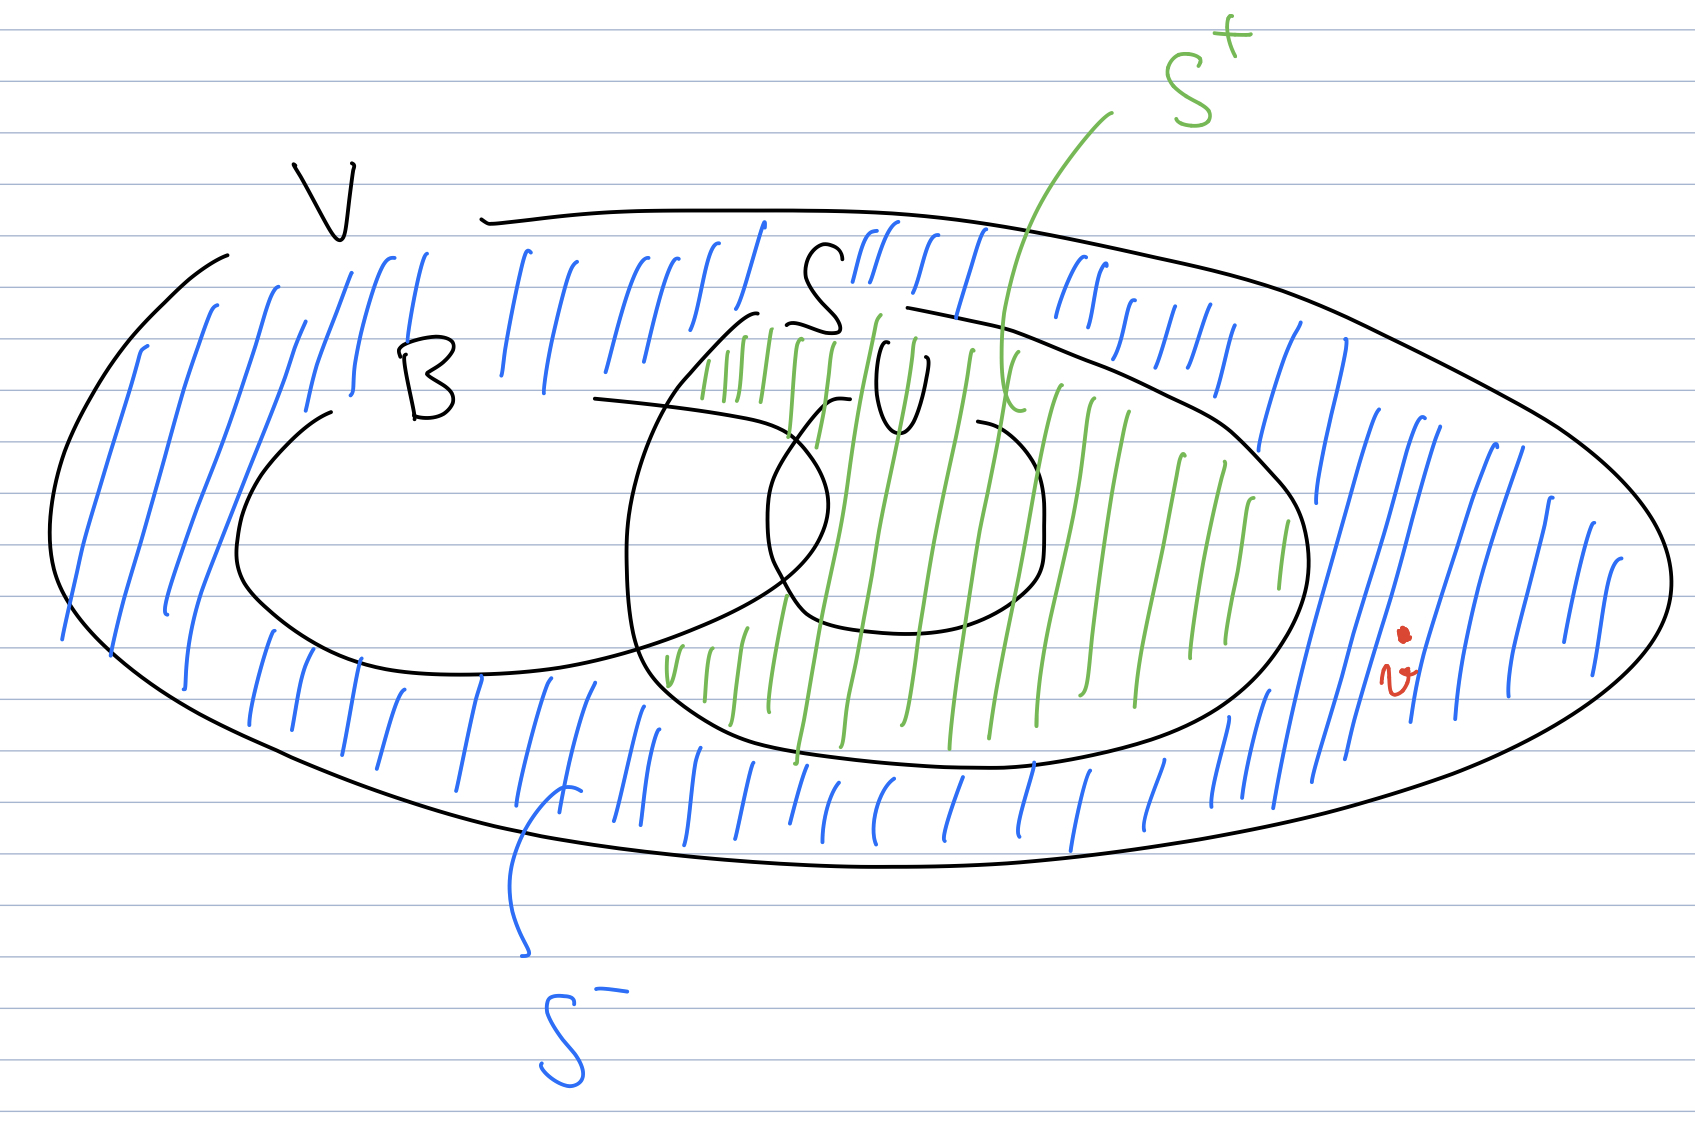
\includegraphics[width=.5\linewidth]{img/lemma_for_every_intact_node.jpeg}
    \caption{Lemma~\ref{lemma_for_every_intact_node}}
    \label{fig:lemma_for_every_intact_node}
\end{figure}

\begin{lem}\label{lemma_for_every_intact_node}
    Let $\ev{V, Q}$ be an FBAS with quorum intersection.
    Let $B$ denote the set of befouled nodes.
    Let $U$ be a quorum containing an intact node, and let $S$ be a set containing $U$.
    Let $S^{+}$ be the set of intact nodes in $S$, and let $S^{-}$ be the set of intact nodes not in $S$.
    Either $S^{-} = \emptyset$, or $\exists v \in S^{-}$ such that $S^{+}$ is $v$-blocking.
    (See Figure~\ref{fig:lemma_for_every_intact_node}.)
\end{lem}

\begin{proof}
    Note that $S^{+} = S \setminus B$ and $S^{-} = (V \setminus S) \setminus B = (V \setminus B) \setminus S^{+}$.
    If $\exists v \in S^{-}$ such that $S^{+}$ is $v$-blocking, then we are done.

    Suppose that $\forall v \in S^{-}$, $S^{+}$ is not $v$-blocking in $\ev{V, Q}$.
    We want to show that $S^{-} = \emptyset$.

    \begin{itemize}
        \item
            $S^{+}$ and $S^{-}$ form a partition of $V \setminus B$,
        \item
            $S^{+}$ is not $v$-blocking in $\ev{V, Q}$ for any arbitrary $v \in S^{-}$,
    \end{itemize}
    By Theorem~\ref{v_blocking_delete}, $S^{+}$ is not $v$-blocking in $\ev{V, Q}^B$ for any $v \in S^{-}$.
    Since $S^{-} = (V \setminus B) \setminus S^{+}$, $S^{+}$ is not $v$-blocking in $\ev{V, Q}^B$ for any $v \in (V \setminus B) \setminus S^{+}$.
    By applying Theorem~\ref{quorum_availability_v_blocking} to the FBAS $\ev{V, Q}^B$ and subset $S^{+}$, $\ev{V, Q}^B$ enjoys quorum availability despite $S^{+}$.

    By the definition of quorum availability(Definition~\ref{def_quorum_availability}), $(V \setminus B) \setminus S^{+}$ is a quorum in $\ev{V, Q}^B$, or $V \setminus B = S^{+}$.
    Suppose $(V \setminus B) \setminus S^{+}$ is a quorum in $\ev{V, Q}^B$.
    This leads to two contradictory claims:
    \begin{itemize}
        \item
            Claim 1: $\ev{V, Q}$ enjoys quorum intersection despite $B$.
            \begin{itemize}
                \item
                    Since $\ev{V, Q}$ enjoys quorum intersection, $B$ is a DSet by Theorem~\ref{befouled_dset}.
                    By the definition of a DSet(Definition~\ref{def_dset}), $\ev{V, Q}^B$ enjoys quorum intersection.
            \end{itemize}
        \item
            Claim 2: $\ev{V, Q}$ does not enjoy quorum intersection despite $B$.
            \begin{itemize}
                \item
                    $U \setminus B$ is nonempty since $U$ contains an intact node.
                    Thus $U \setminus B$ is a quorum in $\ev{V, Q}^B$ by Theorem~\ref{quorum_delete_fbas}.
                    We also assumed that $(V \setminus B) \setminus S^{+}$ is a quorum in $\ev{V, Q}^B$.
                    \begin{align*}
                        (U \setminus B) \cap ((V \setminus B) \setminus S^{+})
                            &= (U \setminus B) \cap S^{-} \\
                            &\subset (S \setminus B) \cap S^{-} \\
                            &\subset S^{+} \cap S^{-} \\
                            &= \emptyset.
                    \end{align*}
                    Therefore, $\ev{V, Q}^B$ does not enjoy quorum intersection.
            \end{itemize}
    \end{itemize}
    Therefore, $(V \setminus B) \setminus S^{+}$ must not be a quorum in $\ev{V, Q}^B$, so $V \setminus B$ must be $S^{+}$.
    In other words, $S^{+}$ contains all the intact nodes, so $S^{-} = \emptyset$, which is exactly what we wanted to show.
\end{proof}

\begin{thm}\label{all_intact_nodes_accept_confirm_same_things}
    If an intact node in an FBAS $\ev{V, Q}$ with quorum intersection confirms a statement $a$, then every intact node will accept and confirm $a$ once sufficient messages are delivered.
\end{thm}

\begin{proof}
    Let $B$ denote the set of befouled nodes.
    When an intact node confirms $a$, some quorum containing such an intact node confirms $a$.
    In other words, there exists a quorum $U \not\subset B$ such that every node in $U$ broadcast that it accepted $a$.
    Some nodes may decide to accept $a$ upon hearing that nodes in $U$ broadcast that it accepted $a$.
    This may, in turn, make more nodes accept $a$.
    Thus we may experience a gradual increase in the number of nodes that accept $a$ over time.
    Since $V$ only contains finitely many nodes, there will be a point at which the number of nodes that accept $a$ stops increasing.
    Let $S$ be the set of nodes that accept $a$ at that point.
    We claim that $S$ contains all intact nodes.

    \begin{itemize}
        \item
            $U$ is a quorum containing an intact node.
        \item
            $U \subset S \subset V$ because every node in $U$ accepted $a$ in the beginning.
        \item
            Let $S^{+} = S \setminus B$ be the set of intact nodes in $S$, and let $S^{-} = (V \setminus S) \setminus B$ be the set of intact nodes not in $S$.
    \end{itemize}
    By Lemma~\ref{lemma_for_every_intact_node}, $S^{-}$ is empty, or $S^{+}$ is $v$-blocking for some $v \in S^{-}$.
    Suppose $S^{-}$ is nonempty.
    Then $v$ accepts $a$ because $S^{+}$ is $v$-blocking and every element of $S^{+}$ broadcast that it has accepted $a$.
    This is a contradiction because we assumed that the number of nodes that accept $a$ stopped increasing.
    Therefore, $S^{-}$ must be empty.
    If $S^{-}$ is empty, then that implies that every intact node accepted and confirmed $a$ assuming sufficient messages are delivered because

    \begin{itemize}
        \item
            Since $S^{-}$ is empty, $S^{+}$ contains all intact nodes in $V$.
            $S^{+} \subset S$, so $S$ contains all intact nodes.
            Since every node in $S$ accepted $a$, every intact node accepted $a$.
        \item
            Since $\ev{V, Q}$ enjoys quorum intersection, $B$ is a DSet by Theorem~\ref{befouled_dset}.
            By the definition of a DSet, $V \setminus B$ is a quorum.
            In other words, the set of all intact nodes is a quorum.
        \item
            Since $V \setminus B$ is a quorum in which every node accepted $a$, every intact node confirmed $a$.
    \end{itemize}
\end{proof}

\newpage
\section{Stellar Consensus Protocol}
\pagebreak
\subsection{Nomination Protocol}

Nomination is done through voting, accepting, and confirming a special type of statement in the form of \textit{nominate $x$}.

\begin{defn}[Nominate]
    A node $v$ is said to nominate a value $x$ if and only if it votes for the statement \textit{nominate $x$}.
\end{defn}

\begin{defn}[Candidate]
    A node $v$ considers a value $x$ to be a candidate if and only if $v$ has confirmed the statement \textit{nominate $x$}.
    Alternatively, we say that a node $v$ has a candidate value $x$.
\end{defn}

\begin{defn}[Weight, Neighbors, and Priority]
    Let $H$ be a cryptographic hash function whose range can be interpreted as a set of integers $\{ 0, \cdots, h_{\max} - 1 \}$.
    Let $G_i(m) = H(i, x_{i - 1}, m)$ be a slot-specific hash function for slot $i$, where $x_{i - 1}$ is the value chosen for the slot preceding $i$.
    Let $N, P$ are arbitrary constants.
    (In Stellar Core, $N, P$ are always set to be $1, 2$.)
    For each round $n$, each node $v$, we define
    \begin{align*}
        \weight(v, v') &= \frac{\abs{\{ q \in Q(v) \mid v' \in q \}}}{\abs{Q(v)}} \\
        \neighbors(v, n) &= \{ v' \mid G_i(N, n, v') < h_{\max} \cdot \weight(v, v') \} \\
        \priority(n, v') &= G_i(P, n, v')
    \end{align*}
\end{defn}

\begin{exmp}[Weight, Neighbors, and Priority(Part 1)]
    \todo[inline,caption={}]{
        proofread!
    }
    We will calculate weight, neighbors, and priority for $v_5$ in Figure~\ref{fig:tiered_quorum_example} as an example.
    Since each quorum slice consists of $v_5$ along with two nodes from $\{ v_1, v_2, v_3, v_4 \}$ as in
    \begin{align*}
        Q(v_5) &= \{ \{ v_1, v_2, v_5 \}, \{ v_1, v_3, v_5 \}, \{ v_1, v_4, v_5 \}, \cdots, \{ v_3, v_4, v_5 \} \},
    \end{align*}
    $Q(v_5)$ has $\binom{4}{2} = 6$ slices.

    We will first calculate the weight of $v_1$.
    \begin{align*}
        \weight(v_5, v_1)
            &= \frac{\abs{\{ q \in Q(v_5) \mid v_1 \in q \}}}{\abs{Q(v_5)}} \\
            &= \frac{\abs{ \{ v_1, v_2, v_5 \}, \{ v_1, v_3, v_5 \}, \{ v_1, v_4, v_5 \}}}{6} \\
            &= \frac{3}{6} = \frac{1}{2}.
    \end{align*}
    By symmetry, $\weight(v_5, v_i) = \frac{1}{2}$ for each $i = 1, 2, 3, 4$.
    $\weight(v_5, v_5) = 1$ because every quorum slice in $Q(v_5)$ contains $v_5$.
    Finally, $\weight(v_5, v_i) = 0$ for all $i = 6, 7, 8, 9, 10$ because no quorum slice in $Q(v_5)$ contains any of $v_6, v_7, \cdots, v_{10}$.
    Therefore, we obtain the following table:
    \begin{center}
      \begin{tabular}{ | c | c | }
        \hline
          $v_i$ & $\weight(v_5, v_i)$ \\ \hline \hline
          $i = 1, 2, 3, 4$ & $1 / 2$ \\ \hline 
          $i = 5$ & 1 \\ \hline 
          $i = 6, 7, 8, 9, 10$ & 0 \\
        \hline
      \end{tabular}
    \end{center}

    For this example, we will suppose that $h_{max} = 100$.
    Let $N, P, i, n$ be fixed.
    Then we will calculate the neighbors.
    First, we will start with $v_1, v_2, v_3, v_4$.

    Suppose
    \begin{align*}
        G_i(N, n, v_1) &= 41 \\
        G_i(N, n, v_2) &= 72 \\
        G_i(N, n, v_3) &= 19 \\
        G_i(N, n, v_4) &= 84.
    \end{align*}
    The condition for a node $v'$ to be in $\neighbors(v_5, n)$ is $G_i(N, n, v') < 100 \cdot \weight(v_5, v')$.
    Therefore, $v_1, v_3 \in \neighbors(v_5, n)$.
    (e.g., $G_i(N, n, v_1) = 41 < 50 = 100 \cdot 1/2 = 100 \cdot \weight(v_5, v_1)$.)

    Moreover, $v_5 \in \neighbors(v_5, n)$ since $\weight(v_5, v_5) = 1$.
    Finally, $v_i \in \neighbors(v_5, n)$ for each $i = 6, 7, \cdots, 10$ because $\weight(v_5, v_i) = 0$.

    Therefore, we have
    \begin{align*}
        \neighbors(v_5, n) = \{ v_1, v_3, v_5 \}.
    \end{align*}
    This is a reasonable choice of neighbors because
    \begin{itemize}
        \item
            $v_5$ trusts $v_1, \cdots, v_4$, so it is a good thing that we have $v_1, v_3$ in $\neighbors(v_5, n)$.
        \item
            $v_5$ trusts $v_5$.
        \item
            Since $v_5$ does not trust $v_6, \cdots, v_{10}$, $v_5$ has no quorum slice containing any of them.
            Thus it is a good thing that $\neighbors(v_5, n)$ does not contain any of them.
    \end{itemize}

    Finally, suppose
    \begin{align*}
        \priority(n, v_1) &= G_i(P, n, v_1) = 17 \\
        \priority(n, v_3) &= G_i(P, n, v_3) = 86 \\
        \priority(n, v_5) &= G_i(P, n, v_5) = 25.
    \end{align*}

    Then $v_5$ will simply nominate the same value as $v_3$.
\end{exmp}

\begin{rem}
    $ $
    \begin{itemize}
        \item
            $\weight$ is not symmetric in general.
            In other words, $\weight(v_i, v_j) \ne \weight(v_j, v_i)$ in general.
        \item
            $\neighbors(v_i)$ is a set of nodes calculated locally at each $v_i$.
            In general, $\neighbors(v_i) \ne \neighbors(v_j)$ for any $i \ne j$.
        \item
            $\priority(n, v)$ is \textit{global} in a sense that the values of $\priority(n, v)$ calculated at node $w$ and $w'$ must be identical for it only depends on $n$, the hash function $G_i$ and the constant $P$.
    \end{itemize}
\end{rem}

\begin{exmp}[Weight, Neighbors, and Priority(Part 2)]
    Suppose that $\priority(n, v_i) = G_i(P, n, v_i)$ for each $i$ is as follows:
    \begin{center}
      \begin{tabular}{ | c | c | c | c | c | c | c | c | c | c | c | }
        \hline
            $i$ & 1 & 2 & 3 & 4 & 5 & 6 & 7 & 8 & 9 & 10 \\ \hline
            $\priority(n, v_i)$ &  26 & 3 & 60 & 89 & 18 & 56 & 35 & 19 & 61 & 27\\
        \hline
      \end{tabular}
    \end{center}
    Moreover, suppose that each node's neighbors is as follows:
    \begin{center}
      \begin{tabular}{ | c | c | }
        \hline
            $i$ & $\neighbors(v_i)$ \\ \hline
            1 & $\{ v_1, v_3 \}$ \\ \hline
            2 & $\{ v_1, v_4 \}$ \\ \hline
            3 & $\{ v_2, v_3, v_4 \}$ \\ \hline
            4 & $\{ v_1, v_2, v_4 \}$ \\ \hline
            5 & $\{ v_2, v_5 \}$ \\ \hline
            6 & $\{ v_1, v_3, v_6\}$ \\ \hline
            7 & $\{ v_1, v_2, v_3, v_7 \}$ \\ \hline
            8 & $\{ v_3, v_8 \}$ \\ \hline
            9 & $\{ v_6, v_7, v_8, v_9 \}$ \\ \hline
            10 & $\{ v_{10} \}$ \\
        \hline
      \end{tabular}
    \end{center}

    Then each node's leader (the node whose nominations it will renominate) will be as follows:
    \begin{center}
      \begin{tabular}{ | c | c | c | c | c | c | c | c | c | c | c | }
        \hline
            $i$ & 1 & 2 & 3 & 4 & 5 & 6 & 7 & 8 & 9 & 10 \\ \hline
            $v_i$'s leader & $v_3$ & $v_4$ & $v_4$ & $v_4$ & $v_5$ & $v_3$ & $v_3$ & $v_3$ & $v_9$ & $v_{10}$ \\
        \hline
      \end{tabular}
    \end{center}

    \begin{figure}[!htb]
        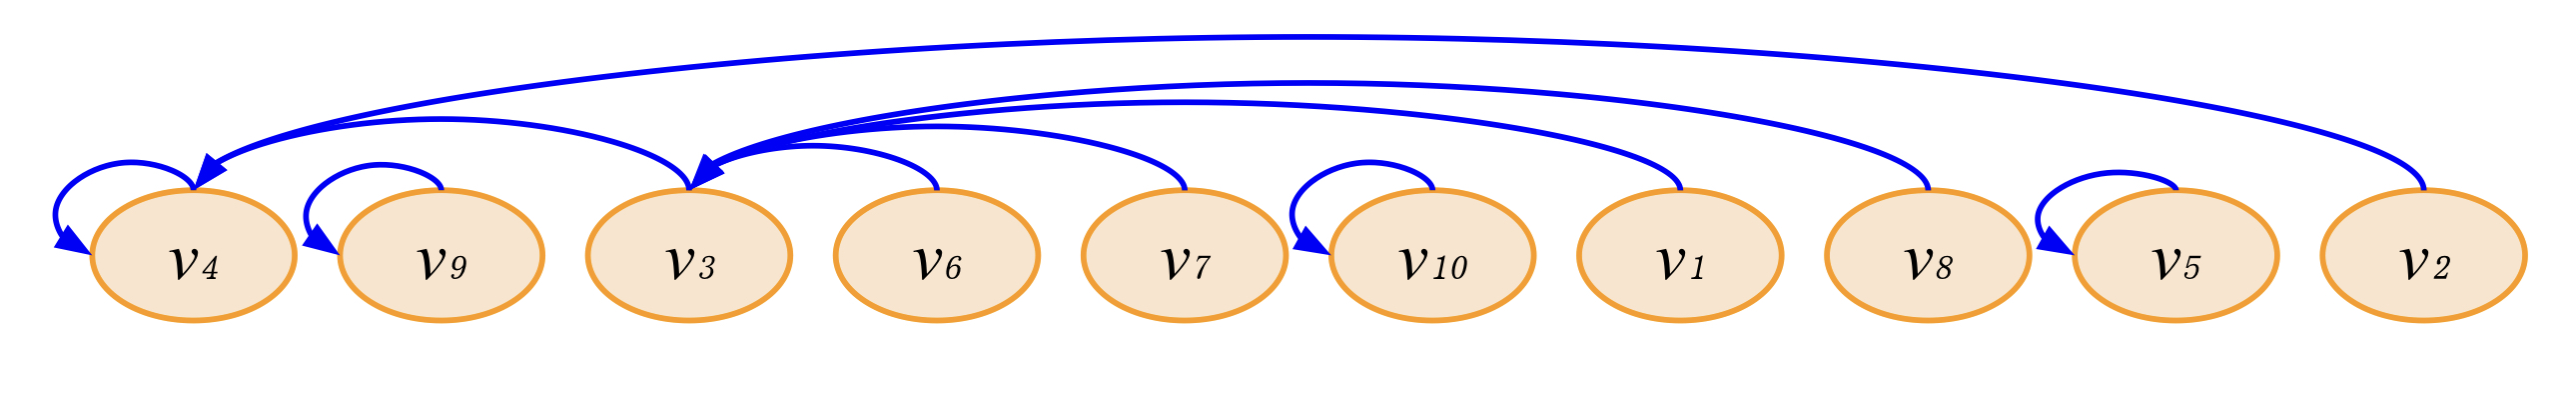
\includegraphics[width=.8\linewidth]{img/leader_election.jpeg}
        \caption{Leader Relation Graph}
        \label{fig:leader_relation}
    \end{figure}

    As you can see, this is a directed graph such that the only cycles are self-loops.
    In this particular case, $v_4, v_9, v_{10}, v_5$ will produce new values, and other nodes will simply renominate those values.
\end{exmp}

\newpage
\subsection{Ballot Protocol}

\end{document}
